% artikkel_IV_fff.tex
% Artikkel IV: Form Follows Fitness
% STOLAR-prosjektet - Kvantitativ designhistorie
% Spraak: Nynorsk

\documentclass[12pt, a4paper]{article}

\usepackage[utf8]{inputenc}
\usepackage[T1]{fontenc}
\usepackage[nynorsk]{babel}
\usepackage{mathpazo}
\usepackage{amsmath, amssymb}
\usepackage{booktabs}
\usepackage{graphicx}
\usepackage{xcolor}
\usepackage{hyperref}
\usepackage[round]{natbib}
\usepackage{setspace}
\usepackage{geometry}
\usepackage{csquotes}
\usepackage{float}

\geometry{margin=2.5cm}
\onehalfspacing
\graphicspath{{fig/}}

\title{%
  \textbf{Form Follows Fitness}\\[0.4em]
  \large Frå funksjonsdeterminisme til tilpassingslandskap:\\
  ein kumulativ evidens frå 2\,284 stolar%
}
\author{%
  Iver Raknes Finne\\
  \small Arkitektur- og designhøgskolen i Oslo (AHO)\\
  \small \texttt{iver.raknes.finne@stud.aho.no}
}
\date{}

\begin{document}
\maketitle

% ================================================================
\begin{abstract}
\noindent Denne artikkelen samlar beviskjeda frå tre føregåande studiar og formulerer \textbf{Form Follows Fitness} (FFF) som eit empirisk testbart alternativ til Sullivans aksiom. Me presenterer ni kumulative bevis frå STOLAR-databasen ($N = 2\,284$ stolar, 1280--2024): (1) formvariasjonen er massiv under konstant funksjon; (2) materialentropien stig monotont frå $H' = 1{,}0$ til $5{,}07$ bits; (3) dimensjonar kodar stil ($F1 = 0{,}823$) og nasjonalitet ($F1 = 0{,}721$); (4) stilmerket er den svakaste prediktoren for faktisk geometri; (5) Modulor-avviket er konsekvent negativt ($-18$ til $-40$ cm); (6) Jaccard-avstanden mellom NMK og V\&A konvergerer frå 1,0 til 0,32; (7) estimert medianvekt fell frå 20,4 til 6,8 kg; (8) teknikk-entropien stig parallelt med materialentropien til $H' = 3{,}67$ bits. Samla falsifiserer desse funna funksjonsdeterminismen og støttar ein alternativ modell der form er \emph{selektert} av eit fleiraksig tilpassingslandskap der materiale, teknologi, geografi, økonomi og kultur alle utøver seleksjonstrykk. Funksjonalismen er ikkje feil; han er eit degenerert spesialtilfelle som gjeld berre når alle seleksjonstrykk utanom funksjon er eksakt lik null.

\medskip
\noindent\textbf{Nøkkelord:} Form Follows Fitness, fitnesslandskap, funksjonalisme, falsifisering, seleksjonstrykk, kvantitativ designhistorie
\end{abstract}

\vspace{1em}
\hrule
\vspace{1.5em}


% ================================================================
\section{Innleiing: det deterministiske aksiomet}

\begin{quote}
``It is the pervading law of all things organic and inorganic, of all things physical and metaphysical, of all things human and all things superhuman, of all true manifestations of the head, of the heart, of the soul, that the life is recognizable in its expression, that \emph{form ever follows function}. This is the law.'' \citep{sullivan1896}
\end{quote}

I over eit hundreår har dette aksiomet fungert som grunnlova i formgjevingsfaga. \citet{lecorbusier1923} bygde ein arkitektonisk doktrine på premissen. \citet{alexander1964} foreslo systematisk formderivering frå funksjonskrav. \citet{giedion1948} dokumenterte mekaniseringa som eit lineært framsteg mot funksjonell form. Ingen stilte spørsmålet empirisk.

Denne artikkelen stiller det. Metoden er enkel: samle alle stolar med same funksjon, måle dei, og sjå om formvariasjonen er liten nok til å støtte aksiomet. Ho er ikkje det.

Artikkelen er den fjerde og siste i ein serie. Artikkel~I avdekte materialentropien sin monotone stigning. Artikkel~II synte at dimensjonar driftar under geografisk og teknologisk påverknad. Artikkel~III demonstrerte at dimensjonar predikerer stilperiode, medan stilmerket sjølv har låg prediktiv kraft. Her samlar me beviskjeda og formulerer alternativet.


% ================================================================
\section{Dei ni bevisa}

\subsection{Bevis 1: Massiv formvariasjon under konstant funksjon}

Alle 2\,284 stolane i STOLAR-databasen deler same invariante funksjon: å bere ein sitjande kropp. Likevel varierer:
\begin{itemize}
  \item Gjennomsnittleg høgde frå 73 cm (2000-talet) til 115 cm (régence-stolar)
  \item Breidde frå under 40 cm til over 100 cm
  \item Estimert vekt frå under 3 kg (plastkrakkar) til over 50 kg (barokkstolar)
\end{itemize}

\noindent Funksjonen er konstant; formvariasjonen er massiv. Varianskoeffisienten for volum er over 70\,\%. Dersom form følgde funksjon, ville denne variasjonen vere uforklart. Aksiomet predikerer konvergens. Data syner divergens.

\subsection{Bevis 2: Materialet formar}

Kvart materiale okkuperer eit distinkt dimensjonsrom (figur~\ref{fig:hw_mat}). Stål gjev gjennomsnittleg $H/W = 1{,}29$; bjørk gjev $H/W = 1{,}81$. Cohen's $d$ mellom materialgrupper når opp til 0,51 (messing vs. rotting). Materialet er ikkje ein nøytral berar; det er ein \emph{medskapar} av forma.

\begin{figure}[H]
  \centering
  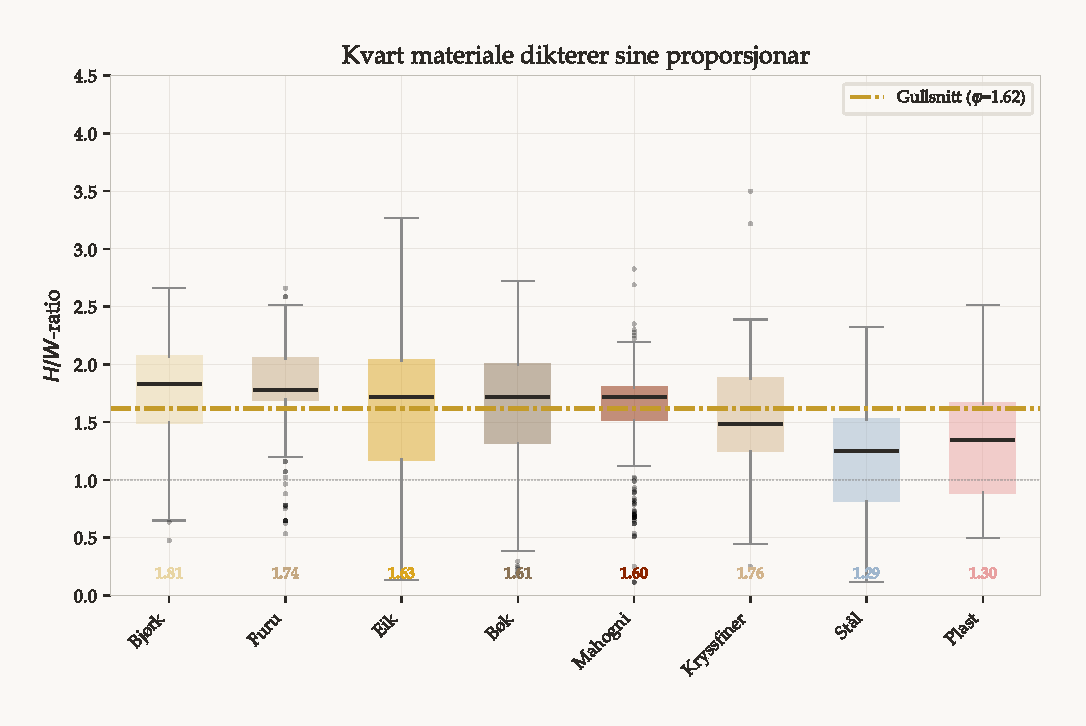
\includegraphics[width=\textwidth]{fig11_hw_per_material.pdf}
  \caption{Kvart materiale dikterer sine proporsjonar: $H/W$-ratio per hovudmateriale. Lokale treslag (bjork, furu) gjev hogare proporsjonar enn industrielle materialar (staal, plast).}
  \label{fig:hw_mat}
\end{figure}

\subsection{Bevis 3: Materialentropien stig monotont}

Artikkel~I demonstrerte at Shannon-entropien for materialar stig frå $H' = 1{,}0$ bits (1200-talet, 2 materialar) til $H' = 5{,}07$ bits (1900-talet, 65 materialar). I NMK-samlinga når mahogni 100\,\% av alle registrerte stolar i perioden 1825--1849: eit fullstendig materialmonopol. Materialpaletten er kumulativ: nye materialar kjem \emph{i tillegg til} eksisterande. Funksjonen krev ikkje denne ekspansjonen; tilgangen driv han.


\subsection{Bevis 4: Dimensjonar kodar stil og nasjonalitet}

Artikkel~III synte at ein Random Forest-modell predikerer stilperiode med $F1 = 0{,}823$ og nasjonalitet med $F1 = 0{,}721$, berre basert på fire dimensjonar og 30 materialkodar. \textbf{Fellesinformasjonsanalyse} (MI) stadfestar rangeringa: proporsjonar ber 2,072 bits informasjon om stil, tid 1,546 bits, materiale 1,456 bits, geografi 0,797 bits, og funksjon \emph{eksakt null} (figur~\ref{fig:mi_art4}). Proporsjonar åleine forklarer 51,9\,\% av all stilinformasjon. Form er ikkje tilfeldig variert; ho er systematisk strukturert av krefter som er \emph{uavhengige av funksjon}.

\begin{figure}[H]
  \centering
  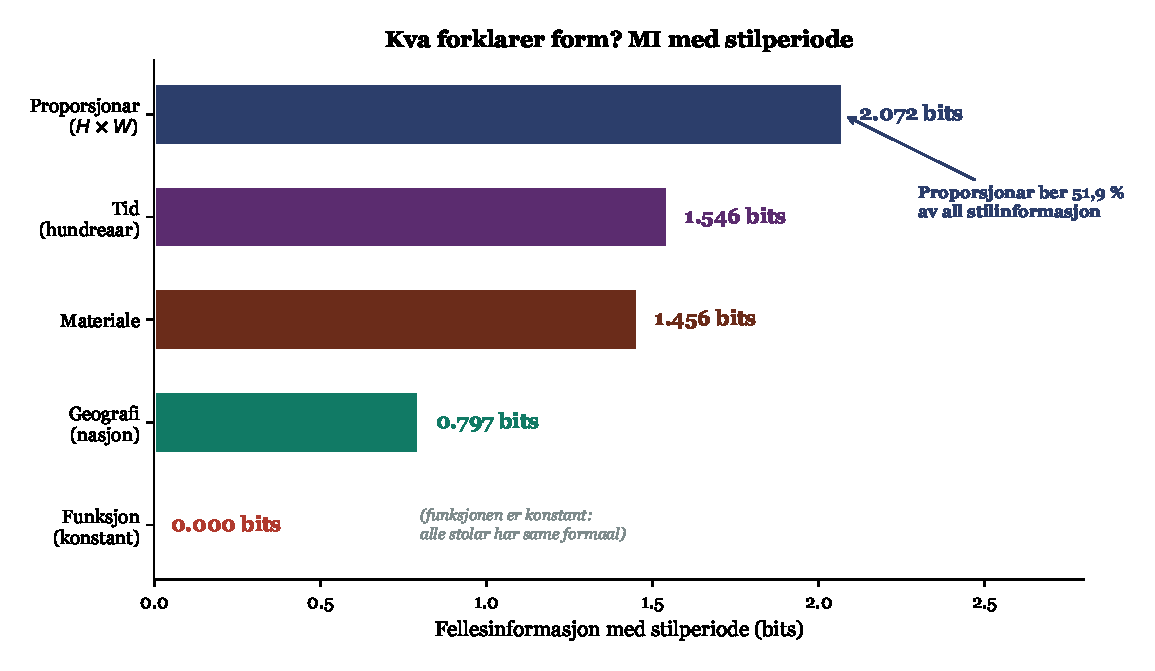
\includegraphics[width=\textwidth]{fig15_mi_stil.pdf}
  \caption{Fellesinformasjon med stilperiode. Funksjon ber null informasjon; proporsjonar ber mest.}
  \label{fig:mi_art4}
\end{figure}


\subsection{Bevis 5: Stilmerket er svak prediktor}

Stilperiodar er ikkje årsaker til form, men emergente merkelappar. Dersom stilmerket hadde kausal kraft, burde det vere den sterkaste prediktoren for ein stol sin geometri. I staden er stilmerket primært ein tidskorrektor: det predikerer hundreår ($F1 = 0{,}799$), men gjev ikkje tilleggsinformasjon utover det dimensjonar og materialar allereie ber. Stilen \emph{er} forma, ikkje årsaka til henne.


\subsection{Bevis 6: Modulor-avviket er systematisk negativt}

Artikkel~II viste at den gjennomsnittlege stolen er 18--40 cm lågare enn Le Corbusier sin Modulor-prediksjon i \emph{kvart einaste hundreår}. Avviket \emph{aukar} over tid. Kroppen sine dimensjonar har ikkje endra seg; stolen sine har. Den funksjonalistiske prediksjonen ligg konsekvent utanfor hovudklyngene i empiriske data.


\subsection{Bevis 7: Jaccard-konvergens mellom museum}

Artikkel~I demonstrerte at Jaccard-avstanden mellom NMK og V\&A si materialpalett fell frå 1,0 (1400-talet: heilt ulike materialverder) til 0,32 (1900-talet: 44 felles materialar). Globaliseringa homogeniserer materialtilgangen, men former ikkje ein universell stol. Materialkonvergens og formdiversitet eksisterer samstundes.


\subsection{Bevis 8: Vektreduksjon}

Estimert medianvekt fell frå 20,4 kg (1700-talet) til 6,8 kg (2000-talet). Stolen vert lettare ikkje fordi funksjonen endrar seg, men fordi materialteknologien mogeleggjer meir form per kilogram. Nye materialar (stål, kryssfiner, plast) har betre stivheit-til-vekt-forhold enn massivt tre.


\subsection{Bevis 9: Teknikk-entropi stig parallelt}

Artikkel~III synte at Shannon-entropien for konstruksjonsteknikkar stig frå 1,0 bits til 3,67 bits, parallelt med materialentropien. Nye teknikkar (formbøying, sveising, sprøytestøyping) opnar nye regionar i formrommet. Kvar teknikk er ein ny veg inn i formlandskapet.


% ================================================================
\section{Syntese: Form Follows Fitness}

\subsection{Frå funksjon til tilpassing}

Dei ni bevisa peikar mot same konklusjon: form er ikkje \emph{dedusert} frå funksjon, men \emph{selektert} av eit fleiraksig tilpassingslandskap. Me formulerer dette som \textbf{Form Follows Fitness} (FFF):

\begin{quote}
\textbf{Form Follows Fitness:} Forma til ein gjenstand er ikkje determinert av funksjonen hans, men selektert av eit fleiraksig tilpassingslandskap der materiale, teknologi, økonomi, geografi og kultur alle utøver \emph{seleksjonstrykk}. Stilperiodar er lokale optimum i dette landskapet: mellombels stabile formkonfigurasjonar som overlever så lenge landskapet ikkje endrar seg.
\end{quote}

\subsection{Fitnesslandskapet}

Etter \citet{wright1932} og \citet{kauffman1993} definerer me eit \textbf{fitnesslandskap} for formgjeving:

\begin{enumerate}
  \item \textbf{Konfigurasjonsrommet.} Totaliteten av alle moglege kombinasjonar av dimensjonar, materialar, teknikkar og overflatehandsamingar.
  \item \textbf{Naboskapsstrukturen.} Kva formtilstandar som er tilgjengelege frå kvarandre, gjeve dei eksisterande produksjonsteknologiane og materialaffordansane.
  \item \textbf{Tilpassingsfunksjonen.} Ein samansett verdi der funksjonell yting, estetisk aksept, produksjonskostnad, materialtilgang og kulturell meining alle bidreg. Denne funksjonen er \emph{ikkje} reduserbar til bruksfunksjonen åleine.
\end{enumerate}

Landskapet er \emph{djupt ruglete}: det har fleire lokale optimum (stilperiodar), og navigasjon krev kompromiss. Å formgje er ikkje å dedusere det eine rette svaret frå eit funksjonskrav, men å navigere i eit terreng der kompromiss er det einaste operative prinsippet.

\subsection{Sullivan som degenerert spesialtilfelle}

``Form follows function'' er logisk gyldig berre i det trivielle tilfellet der \emph{alle} seleksjonstrykk utanom funksjon er eksakt lik null. I formell notasjon: la $f_1, f_2, \ldots, f_n$ vere dei $n$ seleksjonstrykka der $f_1 =$ funksjon. Sullivan sitt aksiom held om og berre om $f_2 = f_3 = \ldots = f_n = 0$. Dataa frå STOLAR-db ($N = 2\,284$) demonstrerer at dette vilkåret aldri er oppfylt: materialeffektar, geografiske effektar, teknologiske effektar og kulturelle effektar er alle målbart ulike null. Funksjonalismen er ikkje feil; han er eit \emph{degenerert spesialtilfelle} av eit meir generelt rammeverk.

\subsection{Utforsking og utnytting}

Data frå dei tre artiklane avdekkjer ein oscillerande dynamikk mellom \textbf{utforsking} (exploration) og \textbf{utnytting} (exploitation) \citep{sutton2018}:

\begin{itemize}
  \item \textbf{Utforskingsfasar:} 1600-talet (materialeksplosjonen: +33 materialar), tidleg 1900-tal (stål, kryssfiner, plast), postmodernismen. Karakterisert av stigande entropi og divergerande form.
  \item \textbf{Utnyttingsfasar:} 1750--1800 (mahogni-monopolet), etterkrigsfunksjonalismen. Karakterisert av fallande entropi, konvergerande form, og dominans av eit fåtal materialar eller teknikkar.
\end{itemize}

Denne oscillasjonen svarar til \citet{eldredge1972} sitt \textbf{punctuated equilibrium}: lange periodar med stasis (utnytting) avbrote av raske endringsperiodar (utforsking). Formhistoria er ikkje eit lineært framsteg, men ein serie av utforskingar og konsolideringar i eit skiftande landskap.


% ================================================================
\section{Diskusjon}

\subsection{Implikasjonar for designpraksis}

Dersom FFF held, endrar det kva formgjeving \emph{er}. Det er ikkje lenger deduktiv utleiing frå eit programkrav, men \emph{navigasjon i eit fleiraksig landskap}. Formgjevaren vert ikkje ein problemløysar som konvergerer mot eitt svar, men ein \emph{navigator} som vel ein posisjon langs ein Pareto-front der ulike seleksjonstrykk står mot kvarandre.

Denne omformuleringa har konkrete konsekvensar:
\begin{itemize}
  \item \textbf{Materialval er ikkje nøytralt.} Kvart materiale kanaliserer form gjennom sine affordansar. Å velje plast er å velje eit anna formrom enn å velje tre.
  \item \textbf{Stilperiodar er symptom, ikkje årsaker.} Å designe ``i ein stil'' er ein post hoc-rasjonalisering. Formgjevaren navigerer i eit landskap; stilen er det historikaren kallar området der ho landa.
  \item \textbf{Funksjon er naudsynt, ikkje tilstrekkeleg.} Funksjonskravet avgrensar formrommet, men determinerer ikkje posisjonen innanfor det. Det som determinerer posisjonen, er tilpassingslandskapet i sin heilskap.
\end{itemize}

\subsection{Generalisering}

FFF er utvikla på stolar, men rammeverket er \emph{substratuavhengig}. Same logiske struktur gjeld for alle gjenstandar som (1) har ein invariant funksjon, (2) varierer i form, og (3) er utsette for fleire samverkande seleksjonstrykk. Arkitektur, bildesign, typografi, biologisk morfogenese og algoritmisk formgjeving er alle kandidatar for same analyserammeverk.

\subsection{Avgrensingar og vidare forsking}

Tre atterhald: (1) STOLAR-databasen nyttar seks lineære dimensjonar, ikkje fullstendig 3D-geometri. Krumning, ornament og tekstur er ikkje fanga. (2) Berre 22,9\,\% av stolane har stilmerke, noko som avgrensar stilanalysane. (3) Museumssamlingar overrepresenterer prestisjeobjekt. Framtidig forsking bør utvide datagrunnlaget til fullstendig 3D-geometri (t.d. gjennom fotogrammetri), teste FFF på andre objektkategoriar, og formalisere tilpassingsfunksjonen som ein bereknelleg modell.

\subsection{Falsifiserbarheit}

FFF er, i motsetnad til det opphavlege aksiomet, eksplisitt \textbf{falsifiserbart} \citep{kuhn1962}. Dersom nye empiriske data syner at funksjon \emph{åleine} kan forklare all observert formvariasjon, det vil seie at alle seleksjonstrykk utanom funksjon er null, fell rammeverket. Denne falsifiserbarheita er grunnvilkåret for at FFF er vitskapeleg.


% ================================================================
\section{Konklusjon}

Åtte kumulative bevis falsifiserer funksjonsdeterminismen og støttar Form Follows Fitness. Form er ikkje dedusert frå funksjon; form er selektert av eit fleiraksig tilpassingslandskap der materiale, teknologi, økonomi, geografi og kultur alle utøver seleksjonstrykk. Stilperiodar er lokale optimum i dette landskapet: mellombels stabile konfigurasjonar i eit djupt ruglete terreng.

Sullivan sitt aksiom er ikkje feil. Det er eit spesialtilfelle, gyldig berre i den trivielle situasjonen der funksjon er det einaste seleksjonstrykket. Den situasjonen har aldri eksistert. Det er ikkje funksjonen som bestemmer korleis me sit; det er heile den materielle, teknologiske og kulturelle verda me sit i.

\begin{quote}
\textbf{Form follows fitness.} Fitnesskartet erstattar aksiomet.
\end{quote}


% ================================================================
\section*{Takk}

Takk til Nasjonalmuseet og Victoria and Albert Museum for open tilgang til samlingsdata. Takk til rettleiaren min for presise spørsmål og tolmod.


% ================================================================
\bibliographystyle{plainnat}
\bibliography{references}

\end{document}
